\documentclass[12pt]{article}
\usepackage[spanish,mexico]{babel}
	\selectlanguage{spanish}
\usepackage{graphicx}
\usepackage{amsmath}
\usepackage{wrapfig}
\usepackage{float}
\usepackage[utf8]{inputenc}
\usepackage{hyperref}
\usepackage{graphicx}
\graphicspath{{images/}}
\setlength{\parskip}{\medskipamount}
\setlength{\parindent}{0pt}
%\usepackage{color}


\usepackage{vmargin}
\setmarginsrb{3 cm}{1.0 cm}{3 cm}{1.0 cm}{1 cm}{1.5 cm}{1 cm}{1.5 cm}
\usepackage{listings}
\usepackage[usenames,dvipsnames]{color}
	\definecolor{ocre}{RGB}{42,105,21}
	\definecolor{ocre2}{RGB}{47,109,130}
	\definecolor{gray2}{gray}{0.95}
	\lstset{
		language=Python,
		backgroundcolor=\color{gray2},
		basicstyle=\color{black}\small\ttfamily, 
		breakatwhitespace=false,         
		breaklines=true,                 
		captionpos=b,                    
		columns=flexible,
		commentstyle=\color{ocre2}\ttfamily, 
		deletekeywords={...},            
		escapeinside={\%*}{*)},          
		extendedchars=true,             
		frame=single,	                 
		keepspaces=true,                 
		keywordstyle=\color{blue}\bfseries,       
		otherkeywords={*,...},          
		numbers=left,                    
		numbersep=5pt,                   
		numberstyle=\tiny, 
		rulecolor=\color{black},         
		showspaces=false,                
		showstringspaces=false,          
		showtabs=false,                  
		stepnumber=1,                    
		stringstyle=\normalfont\color{ocre},     
		tabsize=2,	                     
		title=\lstname                  
		}
\definecolor{labelcolor}{RGB}{100,0,0}

\title{Actividad 9: Aproximación al calculo del periodo del péndulo}
\author{Martin Alejandro Paredes Sosa}
\date{Abril, 2016}

\begin{document}
\maketitle
\section{Introducción}
El calculo del periodo de un péndulo se puede aproximar considerando que $\sin\theta \approx \theta$ para ángulos pequeño, pero este resultado diverge rápidamente para ángulos mayores. Tambien hemos aproximado el periodo por medio de integración numérica y medimos el error relativo al hacer la consideración anterior. Ahora se abordara ese mismo problema del periodo utilizando el álgebra para aproximar el valor.

Como sabemos, el periodo de un péndulo se puede expresar de la siguiente manera:
\begin{equation}\label{T}
T = 4 \sqrt{\frac{l}{2g}} \int^{\theta_0}_0 \frac{1}{\sqrt{\cos\theta - \cos\theta_0}} d\theta
\end{equation}
Si se analiza cuando $\theta_0\rightarrow\pi = \infty$  vemos que la integral diverge, por lo que conviene expresarla de una manera mas simple, como se vera mas adelante.

Si ahora expresamos \eqref{T} como la integral elíptica
\begin{equation} \label{Elip}
F \left(\frac{\pi}{2},k \right) = \int^{\pi/2}_0 \frac{1}{\sqrt{1- k^2 \sin^{2}u}} du
\end{equation}
Y pensamos en series de potencias para aproximar esta integral, podemos comprobar que el periodo se puede aproximar por medio de la siguiente expresión.

\begin{equation}\label{Aprox}
T = 2\pi\sqrt{\frac{l}{g}}\sum^\infty_{n=0} \left[   \left(\frac{(2n!}{(2^nn!)^2} \right) \cdot \sin^2\left( \frac{\theta_0}{2}\right)   \right] 
\end{equation}


\pagebreak
\section{Producto 1}
A partir de \eqref{Aprox}, calculamos los errores relativos al tomar un número finito de términos de la sumatoria. Cada $T_i$ del gráfico representa un desarrollo en serie hasta el i-esimo término. 
Este fue le código que se utilizo para realizar los cálculos.
\lstinputlisting[caption={Código ErrorRe.py}]{ErrorRe.py}
\begin{figure}[H]
\centering
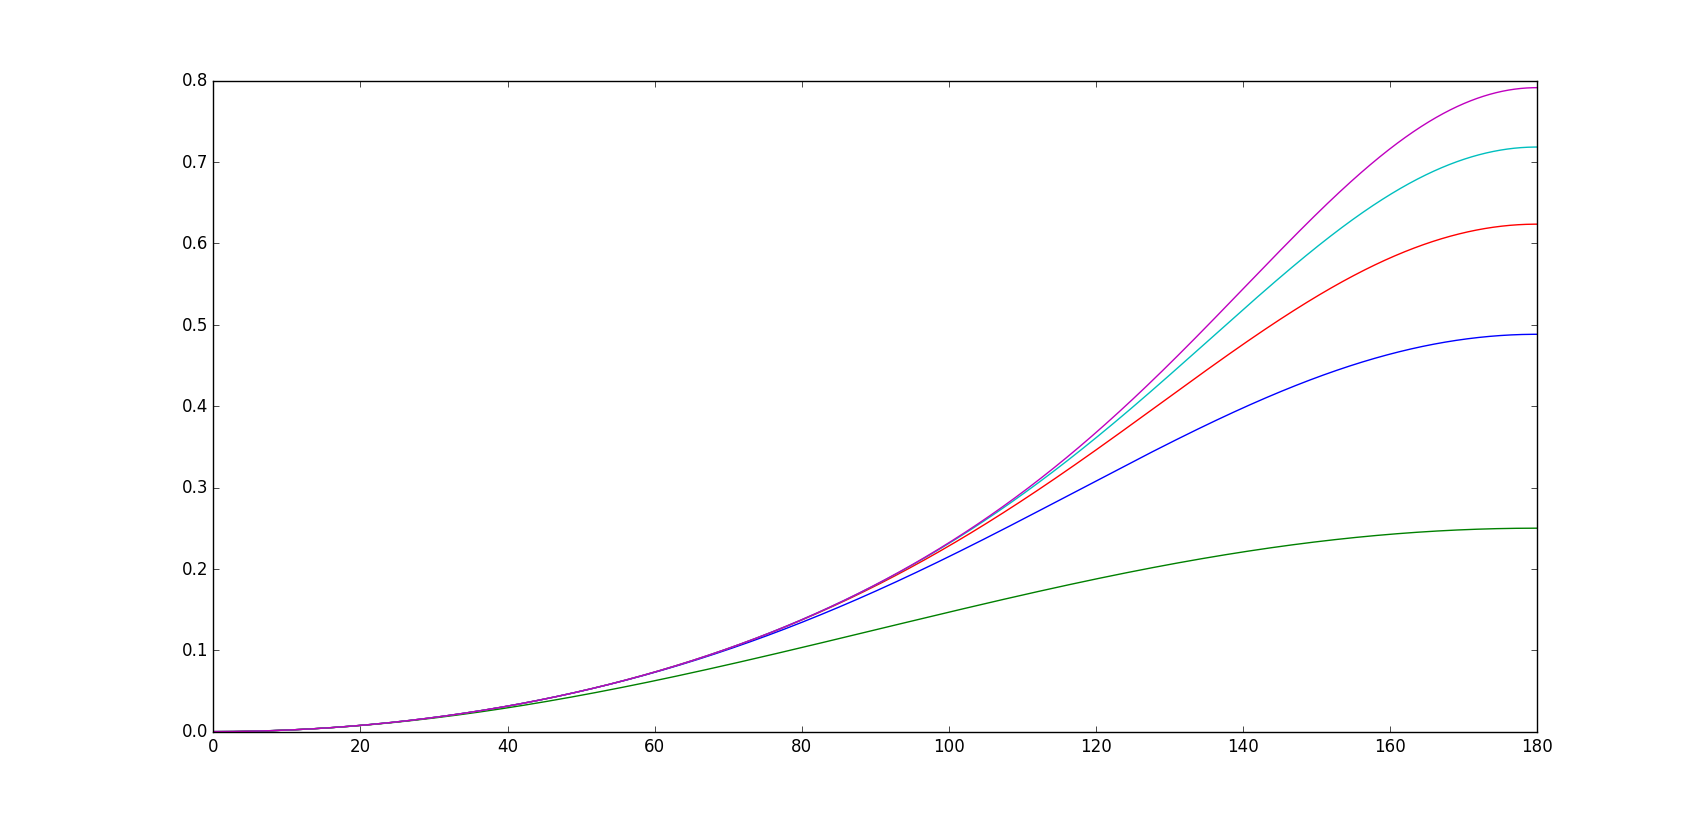
\includegraphics[width=15cm]{Error.png}
\caption{Angulo vs Error relativo}
\end{figure}


\section{Producto 2}
Aplicamos una serie de Maclaurin para $ \sin\left(\frac{\theta_0}{2}\right)$ y trabajando la ecuación \eqref{Elip} llegamos al siguiente resultado:

\noindent
%%%%%%%%%%%%%%%
%%% INPUT:
\begin{minipage}[t]{8ex}\color{red}\bf
(\%i1) 
\end{minipage}
\begin{minipage}[t]{\textwidth}\color{blue}
\begin{verbatim}
/*Función dependiente de K */
Fk1(k) := 1/sqrt(1-(k*sin(u))^2);
\end{verbatim}
\end{minipage}
%%% OUTPUT:
\begin{math}\displaystyle
\parbox{8ex}{\color{labelcolor}(\%o1) }
\mathrm{Fk1}\left( k\right) :=\frac{1}{\sqrt{1-{{\left( k\cdot \mathrm{sin}\left( u\right) \right) }^{2}}}}\mbox{}
\end{math}
\\
%%%%%%%%%%%%%%%
\noindent
%%%%%%%%%%%%%%%
%%% INPUT:
\begin{minipage}[t]{8ex}\color{red}\bf
(\%i2) 
\end{minipage}
\begin{minipage}[t]{\textwidth}\color{blue}
\begin{verbatim}
Desarrollo en serie de Taylor */
taylor(1/sqrt(1-(k*sin(u))^2),u,0,8);
\end{verbatim}
\end{minipage}
%%% OUTPUT:
\begin{math}
\displaystyle
\parbox{8ex}{\color{labelcolor}(\%o2) }
1+\frac{{{k}^{2}}\cdot {{u}^{2}}}{2}+\frac{\left( 9\cdot {{k}^{4}}-4\cdot {{k}^{2}}\right) \cdot {{u}^{4}}}{24}+\frac{\left( 225\cdot {{k}^{6}}-180\cdot {{k}^{4}}+16\cdot {{k}^{2}}\right) \cdot {{u}^{6}}}{720}+\frac{\left( 11025\cdot {{k}^{8}}-12600\cdot {{k}^{6}}+3024\cdot {{k}^{4}}-64\cdot {{k}^{2}}\right) \cdot {{u}^{8}}}{40320}+\mbox{}
\end{math}
\mbox{...}

\noindent
%%%%%%%%%%%%%%%
%%% INPUT:
\begin{minipage}[t]{8ex}\color{red}\bf
(\%i3) 
\end{minipage}
\begin{minipage}[t]{\textwidth}\color{blue}
\begin{verbatim}
/*Definir Fk2 como la expansión de Taylor */
define(Fk2(k),\%);
\end{verbatim}
\end{minipage}
%%% OUTPUT:
\begin{math}
\displaystyle
\parbox{8ex}{\color{labelcolor}(\%o3) }
\mathrm{Fk2}\left( k\right) :=1+\frac{{{k}^{2}}\cdot {{u}^{2}}}{2}+\frac{\left( 9\cdot {{k}^{4}}-4\cdot {{k}^{2}}\right) \cdot {{u}^{4}}}{24}+\frac{\left( 225\cdot {{k}^{6}}-180\cdot {{k}^{4}}+16\cdot {{k}^{2}}\right) \cdot {{u}^{6}}}{720}+\frac{\left( 11025\cdot {{k}^{8}}-12600\cdot {{k}^{6}}+3024\cdot {{k}^{4}}-64\cdot {{k}^{2}}\right) \cdot {{u}^{8}}}{40320}+\mbox{}
\mbox{...}
\end{math}

\noindent
%%%%%%%%%%%%%%%
%%% INPUT:
\begin{minipage}[t]{8ex}\color{red}\bf
(\%i4) 
\end{minipage}
\begin{minipage}[t]{\textwidth}\color{blue}
\begin{verbatim}
/*Definir al sen(theta)*/
define(x(\theta),sin(\theta));
\end{verbatim}
\end{minipage}
%%% OUTPUT:
\begin{math}
\displaystyle
\parbox{8ex}{\color{labelcolor}(\%o4) }
\mathrm{x}\left( \theta\right) :=\mathrm{sin}\left( \theta\right) \mbox{}
\end{math}
%%%%%%%%%%%%%%%

\noindent
%%%%%%%%%%%%%%%
%%% INPUT:
\begin{minipage}[t]{8ex}\color{red}\bf
(\%i5) 
\end{minipage}
\begin{minipage}[t]{\textwidth}\color{blue}
\begin{verbatim}
/*Integramos Fk2 dedes 0 a 90 grados*/
expand(integrate(Fk2(k),u,0,\pi/2));
\end{verbatim}
\end{minipage}
%%% OUTPUT:
\begin{math}
\displaystyle
\parbox{8ex}{\color{labelcolor}(\%o5) }
\frac{35\cdot {{\pi}^{9}}\cdot {{k}^{8}}}{589824}-\frac{5\cdot {{\pi}^{9}}\cdot {{k}^{6}}}{73728}+\frac{5\cdot {{\pi}^{7}}\cdot {{k}^{6}}}{14336}+\frac{{{\pi}^{9}}\cdot {{k}^{4}}}{61440}-\frac{{{\pi}^{7}}\cdot {{k}^{4}}}{3584}+\frac{3\cdot {{\pi}^{5}}\cdot {{k}^{4}}}{1280}-\frac{{{\pi}^{9}}\cdot {{k}^{2}}}{2903040}+\frac{{{\pi}^{7}}\cdot {{k}^{2}}}{40320}-\frac{{{\pi}^{5}}\cdot {{k}^{2}}}{960}+\frac{{{\pi}^{3}}\cdot {{k}^{2}}}{48}+\frac{\pi}{2}\mbox{}
\end{math}
%%%%%%%%%%%%%%%

\noindent
%%%%%%%%%%%%%%%
%%% INPUT:
\begin{minipage}[t]{8ex}\color{red}\bf
(\%i6) 
\end{minipage}
\begin{minipage}[t]{\textwidth}\color{blue}
\begin{verbatim}
/*Sustituimos al sen(theta)*/
subst(x(\theta/2),k,\%);
\end{verbatim}
\end{minipage}
%%% OUTPUT:
\begin{math}
\displaystyle
\parbox{8ex}{\color{labelcolor}(\%o6) }
\frac{35\cdot {{\pi}^{9}}\cdot {{\mathrm{sin}\left( \frac{\theta}{2}\right) }^{8}}}{589824}-\frac{5\cdot {{\pi}^{9}}\cdot {{\mathrm{sin}\left( \frac{\theta}{2}\right) }^{6}}}{73728}+\frac{5\cdot {{\pi}^{7}}\cdot {{\mathrm{sin}\left( \frac{\theta}{2}\right) }^{6}}}{14336}+\frac{{{\pi}^{9}}\cdot {{\mathrm{sin}\left( \frac{\theta}{2}\right) }^{4}}}{61440}-\frac{{{\pi}^{7}}\cdot {{\mathrm{sin}\left( \frac{\theta}{2}\right) }^{4}}}{3584}+\frac{3\cdot {{\pi}^{5}}\cdot {{\mathrm{sin}\left( \frac{\theta}{2}\right) }^{4}}}{1280}-\frac{{{\pi}^{9}}\cdot {{\mathrm{sin}\left( \frac{\theta}{2}\right) }^{2}}}{2903040}+\frac{{{\pi}^{7}}\cdot {{\mathrm{sin}\left( \frac{\theta}{2}\right) }^{2}}}{40320}-\frac{{{\pi}^{5}}\cdot {{\mathrm{sin}\left( \frac{\theta}{2}\right) }^{2}}}{960}+\frac{{{\pi}^{3}}\cdot {{\mathrm{sin}\left( \frac{\theta}{2}\right) }^{2}}}{48}+\frac{\pi}{2}\mbox{}
\end{math}
%%%%%%%%%%%%%%%

\noindent
%%%%%%%%%%%%%%%
%%% INPUT:
\begin{minipage}[t]{8ex}\color{red}\bf
(\%i7) 
\end{minipage}
\begin{minipage}[t]{\textwidth}\color{blue}
\begin{verbatim}
/*Factorizamos*/
expand(\%*2/\pi);
\end{verbatim}
\end{minipage}
%%% OUTPUT:
\begin{math}
\displaystyle
\parbox{8ex}{\color{labelcolor}(\%o7) }
\frac{35\cdot {{\pi}^{8}}\cdot {{\mathrm{sin}\left( \frac{\theta}{2}\right) }^{8}}}{294912}-\frac{5\cdot {{\pi}^{8}}\cdot {{\mathrm{sin}\left( \frac{\theta}{2}\right) }^{6}}}{36864}+\frac{5\cdot {{\pi}^{6}}\cdot {{\mathrm{sin}\left( \frac{\theta}{2}\right) }^{6}}}{7168}+\frac{{{\pi}^{8}}\cdot {{\mathrm{sin}\left( \frac{\theta}{2}\right) }^{4}}}{30720}-\frac{{{\pi}^{6}}\cdot {{\mathrm{sin}\left( \frac{\theta}{2}\right) }^{4}}}{1792}+\frac{3\cdot {{\pi}^{4}}\cdot {{\mathrm{sin}\left( \frac{\theta}{2}\right) }^{4}}}{640}-\frac{{{\pi}^{8}}\cdot {{\mathrm{sin}\left( \frac{\theta}{2}\right) }^{2}}}{1451520}+\frac{{{\pi}^{6}}\cdot {{\mathrm{sin}\left( \frac{\theta}{2}\right) }^{2}}}{20160}-\frac{{{\pi}^{4}}\cdot {{\mathrm{sin}\left( \frac{\theta}{2}\right) }^{2}}}{480}+\frac{{{\pi}^{2}}\cdot {{\mathrm{sin}\left( \frac{\theta}{2}\right) }^{2}}}{24}+1\mbox{}
\end{math}
%%%%%%%%%%%%%%%

\noindent
%%%%%%%%%%%%%%%
%%% INPUT:
\begin{minipage}[t]{8ex}\color{red}\bf
(\%i8) 
\end{minipage}
\begin{minipage}[t]{\textwidth}\color{blue}
\begin{verbatim}
/*Definimos la Funcion que solo depende de theta*/
define(Fk(\theta),\%);
\end{verbatim}
\end{minipage}
%%% OUTPUT:
\begin{math}
\displaystyle
\parbox{8ex}{\color{labelcolor}(\%o8) }
\mathrm{Fk}\left( \theta\right) :=\frac{35\cdot {{\pi}^{8}}\cdot {{\mathrm{sin}\left( \frac{\theta}{2}\right) }^{8}}}{294912}-\frac{5\cdot {{\pi}^{8}}\cdot {{\mathrm{sin}\left( \frac{\theta}{2}\right) }^{6}}}{36864}+\frac{5\cdot {{\pi}^{6}}\cdot {{\mathrm{sin}\left( \frac{\theta}{2}\right) }^{6}}}{7168}+\frac{{{\pi}^{8}}\cdot {{\mathrm{sin}\left( \frac{\theta}{2}\right) }^{4}}}{30720}-\frac{{{\pi}^{6}}\cdot {{\mathrm{sin}\left( \frac{\theta}{2}\right) }^{4}}}{1792}+\frac{3\cdot {{\pi}^{4}}\cdot {{\mathrm{sin}\left( \frac{\theta}{2}\right) }^{4}}}{640}-\frac{{{\pi}^{8}}\cdot {{\mathrm{sin}\left( \frac{\theta}{2}\right) }^{2}}}{1451520}+\frac{{{\pi}^{6}}\cdot {{\mathrm{sin}\left( \frac{\theta}{2}\right) }^{2}}}{20160}-\frac{{{\pi}^{4}}\cdot {{\mathrm{sin}\left( \frac{\theta}{2}\right) }^{2}}}{480}+\frac{{{\pi}^{2}}\cdot {{\mathrm{sin}\left( \frac{\theta}{2}\right) }^{2}}}{24}+1\mbox{}
\end{math}
%%%%%%%%%%%%%%%

\noindent
%%%%%%%%%%%%%%%
%%% INPUT:
\begin{minipage}[t]{8ex}\color{red}\bf
(\%i9) 
\end{minipage}
\begin{minipage}[t]{\textwidth}\color{blue}
\begin{verbatim}
/*Definimos la ecuación del Periodo*/
define(T(theta),(2*pi)*sqrt(l/g)*(Fk(theta)));
\end{verbatim}
\end{minipage}
%%% OUTPUT:
\begin{math}
\displaystyle
\parbox{8ex}{\color{labelcolor}(\%o9) }
\mathrm{T}\left( \theta\right) :=2\pi\sqrt{\frac{l}{g}}\cdot \left(\frac{{{\pi}^{6}}\cdot {{\mathrm{sin}\left( \frac{\theta}{2}\right) }^{2}}}{20160}-\frac{{{\pi}^{4}}\cdot {{\mathrm{sin}\left( \frac{\theta}{2}\right) }^{2}}}{480}+\frac{{{\pi}^{2}}\cdot {{\mathrm{sin}\left( \frac{\theta}{2}\right) }^{2}}}{24}+1+\cdots\right) 
\end{math}

\end{document}
